\section{Mask clustering}

\begin{frame}{What is it?}
The mask clustering algorithm is a clustering algorithm with \emph{SIMD architectures} in mind.

On GPU, it has three stages:

\begin{itemize}
\item Estimation of number of clusters in each module
\item Prefix sum (incremental sum) of estimation
\item Mask clustering
\end{itemize}
\end{frame}

\begin{frame}{Necessary and sufficient condition}
Let's start by the observation that any cluster presents at least one pixel that satisfies the following condition: That the pixels marked with a circle are inactive.

\begin{center}
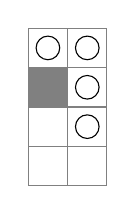
\begin{tikzpicture}[x=5mm, y=5mm]
% Grid
\draw[step=5mm,gray,thin] (0,0) grid (2,4);

% Pixels
\fill[gray] (0,2) rectangle (1,3);

% Circle
\draw (0.5,3.5) circle (1.5mm);
\draw (1.5,3.5) circle (1.5mm);
\draw (1.5,2.5) circle (1.5mm);
\draw (1.5,1.5) circle (1.5mm);
\end{tikzpicture}
\end{center}
\end{frame}

\begin{frame}{Necessary and sufficient condition (2)}
Note: It may be the case that more than one pixel in the cluster satisfies that condition.

\begin{center}
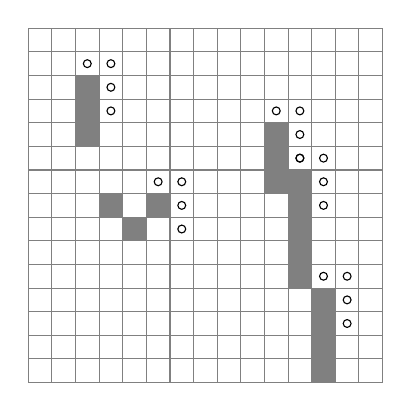
\begin{tikzpicture}[x=3mm, y=3mm]
% Grid
\draw[step=3mm,gray,thin] (0,0) grid (15,15);

% Pixels
\fill[gray] (2,10) rectangle (3,11);
\fill[gray] (2,11) rectangle (3,12);
\fill[gray] (2,12) rectangle (3,13);

\fill[gray] (5,7) rectangle (6,8);
\fill[gray] (4,6) rectangle (5,7);
\fill[gray] (3,7) rectangle (4,8);

\fill[gray] (10,10) rectangle (11,11);
\fill[gray] (10,9) rectangle (11,10);
\fill[gray] (10,8) rectangle (11,9);
\fill[gray] (11,8) rectangle (12,9);
\fill[gray] (11,7) rectangle (12,8);
\fill[gray] (11,6) rectangle (12,7);
\fill[gray] (11,5) rectangle (12,6);
\fill[gray] (11,4) rectangle (12,5);
\fill[gray] (12,3) rectangle (13,4);
\fill[gray] (12,2) rectangle (13,3);
\fill[gray] (12,1) rectangle (13,2);
\fill[gray] (12,0) rectangle (13,1);

% Circle
\draw (2.5,13.5) circle (0.5mm);
\draw (3.5,13.5) circle (0.5mm);
\draw (3.5,12.5) circle (0.5mm);
\draw (3.5,11.5) circle (0.5mm);

\draw (5.5,8.5) circle (0.5mm);
\draw (6.5,8.5) circle (0.5mm);
\draw (6.5,7.5) circle (0.5mm);
\draw (6.5,6.5) circle (0.5mm);

\draw (10.5,11.5) circle (0.5mm);
\draw (11.5,11.5) circle (0.5mm);
\draw (11.5,10.5) circle (0.5mm);
\draw (11.5,9.5) circle (0.5mm);

\draw (11.5,9.5) circle (0.5mm);
\draw (12.5,9.5) circle (0.5mm);
\draw (12.5,8.5) circle (0.5mm);
\draw (12.5,7.5) circle (0.5mm);

\draw (12.5,4.5) circle (0.5mm);
\draw (13.5,4.5) circle (0.5mm);
\draw (13.5,3.5) circle (0.5mm);
\draw (13.5,2.5) circle (0.5mm);
\end{tikzpicture}
\end{center}
\end{frame}

\begin{frame}{Estimation}
In order to do this estimation, given an SP we only require to access the neighbouring SPs on the top, top right, right, bottom right and bottom.

\begin{center}
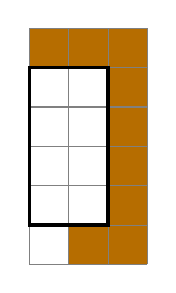
\begin{tikzpicture}[x=5mm, y=5mm]
% Grid

\fill[fill={rgb:red,4;green,2;yellow,1}] (1,-1) rectangle (2,0);
\fill[fill={rgb:red,4;green,2;yellow,1}] (2,-1) rectangle (3,5);
\fill[fill={rgb:red,4;green,2;yellow,1}] (0,4) rectangle (2,5);
\draw[step=5mm,gray,thin] (0,-1) grid (3,5);
\draw[black,very thick] (0,0) -- (2,0) -- (2,4) -- (0,4) -- cycle;
\end{tikzpicture}
\end{center}
\end{frame}

\begin{frame}{Parallel estimation}
This \emph{estimation} algorithm:

\begin{itemize}
\item Overestimates the number of candidates by 1.5~\%
\item Requires 17 bits to compute candidates
\item Can be processed in parallel for all modules and many events at the same time
\item Stores number of candidates into atomic counters
\end{itemize}

The price to pay is that every compute unit that processes an SP will necessarily iterate over all other SPs in the same sensor (raw bank).
\end{frame}

\begin{frame}{Mask clustering (1)}
Let's assume that we have a pixel candidate from the \emph{estimation} algorithm (in green in the figure). The mask clustering begins with loading the following SP quadrant relative to that SP:

\begin{center}
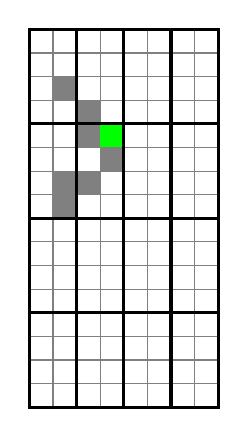
\begin{tikzpicture}[x=3mm, y=3mm]
% Grid
\draw[step=3mm,gray,thin] (0,0) grid (8,16);

% Pixels
\fill[gray] (2,12) rectangle (3,13);
\fill[gray] (2,11) rectangle (3,12);
\fill[gray] (2,9) rectangle (3,10);
\fill[green] (3,11) rectangle (4,12);
\fill[gray] (3,10) rectangle (4,11);
\fill[gray] (1,13) rectangle (2,14);
\fill[gray] (1,9) rectangle (2,10);
\fill[gray] (1,8) rectangle (2,9);

% SPs
\draw[black,very thick] (0,0) -- (2,0) -- (2,4) -- (0,4) -- cycle;
\draw[black,very thick] (0,4) -- (2,4) -- (2,8) -- (0,8) -- cycle;
\draw[black,very thick] (0,8) -- (2,8) -- (2,12) -- (0,12) -- cycle;
\draw[black,very thick] (0,12) -- (2,12) -- (2,16) -- (0,16) -- cycle;

\draw[black,very thick] (2,0) -- (4,0) -- (4,4) -- (2,4) -- cycle;
\draw[black,very thick] (2,4) -- (4,4) -- (4,8) -- (2,8) -- cycle;
\draw[black,very thick] (2,8) -- (4,8) -- (4,12) -- (2,12) -- cycle;
\draw[black,very thick] (2,12) -- (4,12) -- (4,16) -- (2,16) -- cycle;

\draw[black,very thick] (4,0) -- (6,0) -- (6,4) -- (4,4) -- cycle;
\draw[black,very thick] (4,4) -- (6,4) -- (6,8) -- (4,8) -- cycle;
\draw[black,very thick] (4,8) -- (6,8) -- (6,12) -- (4,12) -- cycle;
\draw[black,very thick] (4,12) -- (6,12) -- (6,16) -- (4,16) -- cycle;

\draw[black,very thick] (6,0) -- (8,0) -- (8,4) -- (6,4) -- cycle;
\draw[black,very thick] (6,4) -- (8,4) -- (8,8) -- (6,8) -- cycle;
\draw[black,very thick] (6,8) -- (8,8) -- (8,12) -- (6,12) -- cycle;
\draw[black,very thick] (6,12) -- (8,12) -- (8,16) -- (6,16) -- cycle;
\end{tikzpicture}
\end{center}
\end{frame}

\begin{frame}{Mask clustering (2)}
In order to find all clusters in the vicinity of the green cluster, it is sufficient to create a \textbf{bitmask} with the eight neighbouring pixels and apply it to the pixel array:

\begin{center}
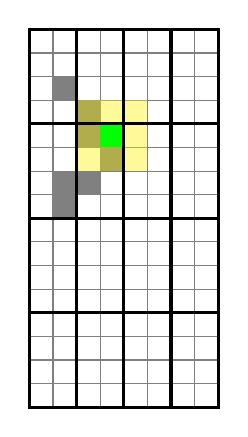
\begin{tikzpicture}[x=3mm, y=3mm]
% Grid
\draw[step=3mm,gray,thin] (0,0) grid (8,16);

% Pixels
\fill[gray] (2,12) rectangle (3,13);
\fill[gray] (2,11) rectangle (3,12);
\fill[gray] (2,9) rectangle (3,10);
\fill[gray] (3,10) rectangle (4,11);
\fill[gray] (1,13) rectangle (2,14);
\fill[gray] (1,9) rectangle (2,10);
\fill[gray] (1,8) rectangle (2,9);

% Bitmask
\fill[yellow,opacity=0.4] (2,10) rectangle (5,13);

\fill[green] (3,11) rectangle (4,12);

% SPs
\draw[black,very thick] (0,0) -- (2,0) -- (2,4) -- (0,4) -- cycle;
\draw[black,very thick] (0,4) -- (2,4) -- (2,8) -- (0,8) -- cycle;
\draw[black,very thick] (0,8) -- (2,8) -- (2,12) -- (0,12) -- cycle;
\draw[black,very thick] (0,12) -- (2,12) -- (2,16) -- (0,16) -- cycle;

\draw[black,very thick] (2,0) -- (4,0) -- (4,4) -- (2,4) -- cycle;
\draw[black,very thick] (2,4) -- (4,4) -- (4,8) -- (2,8) -- cycle;
\draw[black,very thick] (2,8) -- (4,8) -- (4,12) -- (2,12) -- cycle;
\draw[black,very thick] (2,12) -- (4,12) -- (4,16) -- (2,16) -- cycle;

\draw[black,very thick] (4,0) -- (6,0) -- (6,4) -- (4,4) -- cycle;
\draw[black,very thick] (4,4) -- (6,4) -- (6,8) -- (4,8) -- cycle;
\draw[black,very thick] (4,8) -- (6,8) -- (6,12) -- (4,12) -- cycle;
\draw[black,very thick] (4,12) -- (6,12) -- (6,16) -- (4,16) -- cycle;

\draw[black,very thick] (6,0) -- (8,0) -- (8,4) -- (6,4) -- cycle;
\draw[black,very thick] (6,4) -- (8,4) -- (8,8) -- (6,8) -- cycle;
\draw[black,very thick] (6,8) -- (8,8) -- (8,12) -- (6,12) -- cycle;
\draw[black,very thick] (6,12) -- (8,12) -- (8,16) -- (6,16) -- cycle;
\end{tikzpicture}
\end{center}
\end{frame}

\begin{frame}{Mask clustering (3)}
In order to find all clusters in the vicinity of the green cluster, it is sufficient to create a \textbf{bitmask} with the eight neighbouring pixels and apply it to the pixel array:

\begin{center}
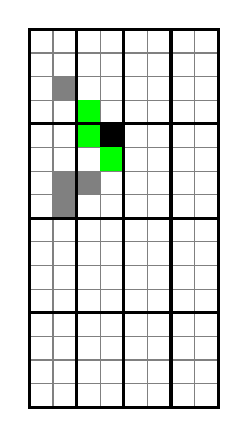
\begin{tikzpicture}[x=3mm, y=3mm]
% Grid
\draw[step=3mm,gray,thin] (0,0) grid (8,16);

% Pixels
\fill[gray] (2,9) rectangle (3,10);
\fill[gray] (1,13) rectangle (2,14);
\fill[gray] (1,9) rectangle (2,10);
\fill[gray] (1,8) rectangle (2,9);

% Forming cluster
\fill[black] (3,11) rectangle (4,12);
\fill[green] (2,12) rectangle (3,13);
\fill[green] (2,11) rectangle (3,12);
\fill[green] (3,10) rectangle (4,11);

% SPs
\draw[black,very thick] (0,0) -- (2,0) -- (2,4) -- (0,4) -- cycle;
\draw[black,very thick] (0,4) -- (2,4) -- (2,8) -- (0,8) -- cycle;
\draw[black,very thick] (0,8) -- (2,8) -- (2,12) -- (0,12) -- cycle;
\draw[black,very thick] (0,12) -- (2,12) -- (2,16) -- (0,16) -- cycle;

\draw[black,very thick] (2,0) -- (4,0) -- (4,4) -- (2,4) -- cycle;
\draw[black,very thick] (2,4) -- (4,4) -- (4,8) -- (2,8) -- cycle;
\draw[black,very thick] (2,8) -- (4,8) -- (4,12) -- (2,12) -- cycle;
\draw[black,very thick] (2,12) -- (4,12) -- (4,16) -- (2,16) -- cycle;

\draw[black,very thick] (4,0) -- (6,0) -- (6,4) -- (4,4) -- cycle;
\draw[black,very thick] (4,4) -- (6,4) -- (6,8) -- (4,8) -- cycle;
\draw[black,very thick] (4,8) -- (6,8) -- (6,12) -- (4,12) -- cycle;
\draw[black,very thick] (4,12) -- (6,12) -- (6,16) -- (4,16) -- cycle;

\draw[black,very thick] (6,0) -- (8,0) -- (8,4) -- (6,4) -- cycle;
\draw[black,very thick] (6,4) -- (8,4) -- (8,8) -- (6,8) -- cycle;
\draw[black,very thick] (6,8) -- (8,8) -- (8,12) -- (6,12) -- cycle;
\draw[black,very thick] (6,12) -- (8,12) -- (8,16) -- (6,16) -- cycle;
\end{tikzpicture}
\end{center}
\end{frame}

\begin{frame}{Mask clustering (4)}
We can then repeat from the new found pixels, until we find no more pixels with this method.

\begin{center}
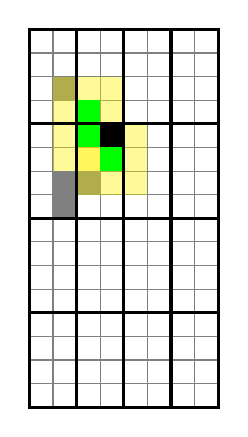
\begin{tikzpicture}[x=3mm, y=3mm]
% Grid
\draw[step=3mm,gray,thin] (0,0) grid (8,16);

% Pixels
\fill[gray] (2,9) rectangle (3,10);
\fill[gray] (1,13) rectangle (2,14);
\fill[gray] (1,9) rectangle (2,10);
\fill[gray] (1,8) rectangle (2,9);

% Bitmask
\fill[yellow,opacity=0.4] (1,10) rectangle (4,14);
\fill[yellow,opacity=0.4] (2,9) rectangle (5,12);

% Forming cluster
\fill[black] (3,11) rectangle (4,12);
\fill[green] (2,12) rectangle (3,13);
\fill[green] (2,11) rectangle (3,12);
\fill[green] (3,10) rectangle (4,11);

% SPs
\draw[black,very thick] (0,0) -- (2,0) -- (2,4) -- (0,4) -- cycle;
\draw[black,very thick] (0,4) -- (2,4) -- (2,8) -- (0,8) -- cycle;
\draw[black,very thick] (0,8) -- (2,8) -- (2,12) -- (0,12) -- cycle;
\draw[black,very thick] (0,12) -- (2,12) -- (2,16) -- (0,16) -- cycle;

\draw[black,very thick] (2,0) -- (4,0) -- (4,4) -- (2,4) -- cycle;
\draw[black,very thick] (2,4) -- (4,4) -- (4,8) -- (2,8) -- cycle;
\draw[black,very thick] (2,8) -- (4,8) -- (4,12) -- (2,12) -- cycle;
\draw[black,very thick] (2,12) -- (4,12) -- (4,16) -- (2,16) -- cycle;

\draw[black,very thick] (4,0) -- (6,0) -- (6,4) -- (4,4) -- cycle;
\draw[black,very thick] (4,4) -- (6,4) -- (6,8) -- (4,8) -- cycle;
\draw[black,very thick] (4,8) -- (6,8) -- (6,12) -- (4,12) -- cycle;
\draw[black,very thick] (4,12) -- (6,12) -- (6,16) -- (4,16) -- cycle;

\draw[black,very thick] (6,0) -- (8,0) -- (8,4) -- (6,4) -- cycle;
\draw[black,very thick] (6,4) -- (8,4) -- (8,8) -- (6,8) -- cycle;
\draw[black,very thick] (6,8) -- (8,8) -- (8,12) -- (6,12) -- cycle;
\draw[black,very thick] (6,12) -- (8,12) -- (8,16) -- (6,16) -- cycle;
\end{tikzpicture}
\end{center}
\end{frame}

\begin{frame}{Mask clustering (5)}
We can then repeat from the new found pixels, until we find no more pixels with this method.

\begin{center}
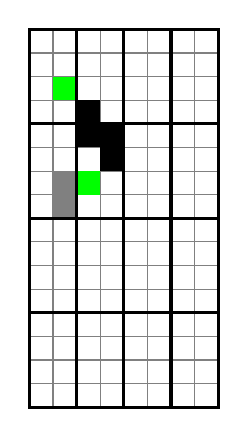
\begin{tikzpicture}[x=3mm, y=3mm]
% Grid
\draw[step=3mm,gray,thin] (0,0) grid (8,16);

% Pixels
\fill[gray] (1,9) rectangle (2,10);
\fill[gray] (1,8) rectangle (2,9);

% Forming cluster
\fill[black] (3,11) rectangle (4,12);
\fill[black] (2,12) rectangle (3,13);
\fill[black] (2,11) rectangle (3,12);
\fill[black] (3,10) rectangle (4,11);
\fill[green] (1,13) rectangle (2,14);
\fill[green] (2,9) rectangle (3,10);

% SPs
\draw[black,very thick] (0,0) -- (2,0) -- (2,4) -- (0,4) -- cycle;
\draw[black,very thick] (0,4) -- (2,4) -- (2,8) -- (0,8) -- cycle;
\draw[black,very thick] (0,8) -- (2,8) -- (2,12) -- (0,12) -- cycle;
\draw[black,very thick] (0,12) -- (2,12) -- (2,16) -- (0,16) -- cycle;

\draw[black,very thick] (2,0) -- (4,0) -- (4,4) -- (2,4) -- cycle;
\draw[black,very thick] (2,4) -- (4,4) -- (4,8) -- (2,8) -- cycle;
\draw[black,very thick] (2,8) -- (4,8) -- (4,12) -- (2,12) -- cycle;
\draw[black,very thick] (2,12) -- (4,12) -- (4,16) -- (2,16) -- cycle;

\draw[black,very thick] (4,0) -- (6,0) -- (6,4) -- (4,4) -- cycle;
\draw[black,very thick] (4,4) -- (6,4) -- (6,8) -- (4,8) -- cycle;
\draw[black,very thick] (4,8) -- (6,8) -- (6,12) -- (4,12) -- cycle;
\draw[black,very thick] (4,12) -- (6,12) -- (6,16) -- (4,16) -- cycle;

\draw[black,very thick] (6,0) -- (8,0) -- (8,4) -- (6,4) -- cycle;
\draw[black,very thick] (6,4) -- (8,4) -- (8,8) -- (6,8) -- cycle;
\draw[black,very thick] (6,8) -- (8,8) -- (8,12) -- (6,12) -- cycle;
\draw[black,very thick] (6,12) -- (8,12) -- (8,16) -- (6,16) -- cycle;
\end{tikzpicture}
\end{center}
\end{frame}

\begin{frame}{Various points}
\begin{itemize}
\item This algorithm requires loading a total of 15 neighbouring SPs
\item It can be processed with 128 bits (currently, implemented as 4 ints)
\item Creating a mask is very cheap: Just eight shifts and some mask for corner cases
\item Each iteration can theoretically find up to 8 neighbouring pixels. Given the candidate conditions, it can actually never find more than 5, which is still pretty good
\end{itemize}
\end{frame}

\begin{frame}{Some other points}
\begin{itemize}
\item The algorithm is highly parallelizable / vectorizable
\item There is a limited number of iterations in order to find all possible candidates. 8 iterations is enough to find $99.9~\%$ of clusters
\item The algorithm is not very readable, it requires a lot of heavy bitmasking
\end{itemize}
\end{frame}

\begin{frame}{Validation}
By construction, this algorithm will not give you the same answer as VPClustering:

\begin{itemize}
\item It finds about $0.07~\%$ more clusters
\item \emph{It does not always find the same expected LHCb IDs}. Note the LHCb ID has the following structure, highly dependent on the average X and Y of the pixels in the cluster:
\end{itemize}

\begin{figure}
\includegraphics[width=250pt]{lhcb_id}
\end{figure}
\end{frame}

\begin{frame}{Validation (2)}
A version of this algorithm (not vectorized yet) has been implemented in Gaudi (branch \emph{dcampora\_vpclus\_bitmask}). The reconstruction efficiency of the tracks produced by Velo tracking drops by 0.5~\%.

This drop in RE is probably due to the slight differences in certain LHCb IDs. The tracks produced are very similar, and their states almost identical.

\begin{center}
\emph{Is it acceptable to find slightly different clusters?}
\end{center}
\end{frame}
